\documentclass[11pt]{article}
\usepackage[margin=1in]{geometry}
\usepackage{amsmath,amssymb}
\usepackage{booktabs}
\usepackage{array}
\usepackage{hyperref}
\usepackage{xcolor}
\usepackage{enumitem}
\usepackage{longtable}
\usepackage{adjustbox}

\setlist[itemize]{leftmargin=*,topsep=2pt,itemsep=2pt}
\setlist[enumerate]{leftmargin=*,topsep=2pt,itemsep=2pt}
\newcommand{\dth}{\Delta\theta}
\newcommand{\pithirty}{$\pi/30$}
\newcommand{\pitwenty}{$\pi/20$}

\title{Phase 6 notes: factored actions and larger-$N$ scaling}
\author{}
\date{Draft notes, updated through  $N=12$ scaled-radius runs}

\begin{document}
\maketitle

\section{Purpose of Phase 6}

The goal of Phase~6 is to separate two issues that were becoming entangled in the larger-$N$ PPO experiments. The first is the growth of the monolithic action space. In the monolithic formulation, the policy chooses one categorical action from all nonzero vectors in $\{-1,0,1\}^N$, so the number of possible actions is $3^N-1$. This becomes large very quickly. For example, $N=6$ already has $728$ monolithic actions, while $N=12$ would have $531{,}440$ nonzero actions.

The second issue is geometric scaling. With fixed bead radius $r=0.05$ and total chain length fixed to one, the adjacent bead spacing is $1/N$. The near-contact threshold used by the environment is $2.2r$. Thus fixed radius becomes geometrically invalid when $1/N < 2.2r$. This occurs at $N=10$, since $1/10=0.1 < 0.11=2.2(0.05)$. Phase~6 therefore uses factored actions to address the action-space problem and then introduces a scaled-radius branch, $r=0.4/N$, to continue beyond the fixed-radius geometric limit.

\section{Factored action representation}

The factored action representation replaces the single large categorical action with one ternary decision per joint:
\begin{equation}
 a_j \in \{-1,0,1\}, \qquad j=1,\ldots,N .
\end{equation}
In the implementation this is a \texttt{MultiDiscrete([3]*N)} action space. The global no-op action is therefore technically available, unlike in the monolithic action list where the all-zero vector was excluded. However, in the successful large-$N$ runs analyzed so far, the measured no-op fraction is zero, so the no-op does not appear to be used by the trained policies.

The PPO hyperparameters were kept the same as in the monolithic sweeps unless otherwise noted: \texttt{MlpPolicy}, $\gamma=0.99$, \texttt{n\_steps=2048}, \texttt{batch\_size=256}, \texttt{n\_epochs=10}, learning rate $3\times 10^{-4}$, \texttt{clip\_range=0.2}, and \texttt{ent\_coef=0}. Since \texttt{ent\_coef=0}, the entropy difference between a monolithic categorical distribution and a multi-categorical factored distribution is not directly rewarded in the PPO objective.

\section{Small-$N$ validation against existing benchmarks}

The first check was whether factored PPO still recovers the known small-$N$ behavior. For $N=3$ and $N=4$, the factored runs were compared with the earlier monolithic PPO sweeps and the Howard policy-iteration benchmarks where available. The overall conclusion is that the factored representation does not break the problem: it recovers positive coherent strokes, and for $N=4$ it remains in essentially the same reward--geometry regime as monolithic PPO and Howard policy iteration.

There was one notable $N=3$, $\dth=\pi/20$ factored failure seed. That seed converged to a coherent periodic cycle with negative mean reward and wrong orientation, rather than to a no-op collapse. Midpoint diagnostics showed two invalid wall-clearance transitions followed by a valid but negative-flux part of the cycle. This appears to be a genuine bad local optimum, not a pathology of the no-op action.

\section{Factored versus monolithic at $N=5$ and $N=6$}

The next test was whether the factored action representation helps once the monolithic action space begins to strain. The $N=5$ factored runs essentially matched the earlier monolithic runs, while the $N=6$ factored runs improved the large-chain scaling behavior.

\begin{table}[htbp]
\centering
\scriptsize
\begin{tabular}{ccccccccc}
\toprule
$N$ & $\dth$ & action & steps & runs & median mean reward & median $\rho$ & typical $L$ & comments \\
\midrule
5 & $\pi/20$ & monolithic & $2\times 10^6$ & 10 & 1.667 & 44.82 & mixed & Phase 5 reference \\
5 & $\pi/20$ & factored   & $2\times 10^6$ & 10 & 1.628 & 45.24 & short & matches monolithic \\
5 & $\pi/30$ & monolithic & $2\times 10^6$ & 10 & 1.003 & 46.09 & mixed & Phase 5 reference \\
5 & $\pi/30$ & factored   & $2\times 10^6$ & 10 & 1.041 & 45.35 & short & matches monolithic \\
\midrule
6 & $\pi/20$ & monolithic & $3\times 10^6$ & 10 & 1.492 & 52.06 & long/mixed & longer closures, more drift \\
6 & $\pi/20$ & factored   & $3\times 10^6$ & 10 & 2.027 & 48.20 & mostly 14--18, one 32 & cleaner and higher reward \\
6 & $\pi/30$ & factored   & $3\times 10^6$ & 10 & 1.395 & 47.69 & mostly 21--25, one 49 & clean positive strokes \\
\bottomrule
\end{tabular}
\caption{Summary of factored versus monolithic PPO at $N=5$ and $N=6$. At $N=5$, factored PPO essentially matches monolithic PPO. At $N=6$, the factored representation gives shorter, cleaner cycles and higher median mean reward, although the median reward-per-area ratio $\rho$ is lower than in the monolithic reference.}
\label{tab:phase6-n5-n6}
\end{table}

The $N=6$ result is the first strong indication that the factored representation is doing useful work. Monolithic $N=6$ could find positive strokes but often produced longer exact-state closures, including cycles near $L=97$ and $L=108$ in the earlier sweep. Factored $N=6$ instead produced compact cycles, mostly between $14$ and $18$ steps at $\dth=\pi/20$, with no wrong-orientation or no-op failures.

\section{Fixed-radius $N=8$ and the geometric limit at $N=10$}

With the factored representation, the fixed-radius branch was pushed to $N=8$ at $\dth=\pi/20$. This run was successful: all ten seeds produced positive coherent strokes, no wrong-orientation failures, and no no-op collapse. Most cycles were short, with several $L=14$ strokes and a few longer commensurate closures.

\begin{table}[htbp]
\centering
\scriptsize
\begin{tabular}{cccccccc}
\toprule
$N$ & $\dth$ & action & radius & steps & runs & median mean reward & median $\rho$ \\
\midrule
8 & $\pi/20$ & factored & 0.05 & $4\times 10^6$ & 10 & 3.004 & 52.29 \\
\bottomrule
\end{tabular}
\caption{Fixed-radius $N=8$ factored PPO sweep. This is still geometrically valid because the adjacent spacing $1/8=0.125$ is larger than the near-contact threshold $2.2(0.05)=0.11$.}
\label{tab:phase6-n8-fixed}
\end{table}

Attempting fixed-radius $N=10$ failed immediately. The no-op state at the reset configuration already receives the wall/contact penalty. This is a geometry issue, not a learning issue. The diagnostic is simple:
\begin{equation}
\hbox{adjacent spacing} = \frac{1}{N}, \qquad
\hbox{near-contact threshold} = 2.2r .
\end{equation}
For $r=0.05$, the threshold is $0.11$. Thus $N=9$ is barely valid because $1/9 \approx 0.1111 > 0.11$, while $N=10$ is invalid because $1/10=0.1 < 0.11$.

A nonadjacent-distance diagnostic on the $N=8$ fixed-radius runs showed that most learned strokes were not being clipped by nonadjacent self-contact. Adjacent distances are close to the threshold by construction, but nonadjacent distances typically remained well above threshold. Thus the $N=8$ result appears to be a meaningful fixed-radius result, while continuing beyond $N=9$ requires changing the geometric scaling.

\section{Scaled-radius branch}

To continue beyond the fixed-radius limit, the radius was scaled with $N$:
\begin{equation}
 r = \frac{0.4}{N} .
\end{equation}
This choice agrees with the fixed-radius value at $N=8$, since $0.4/8=0.05$, and preserves a constant relative thickness as the chain is refined. Under this scaling, the adjacent spacing is $1/N$ and the near-contact threshold is $2.2(0.4/N)=0.88/N$, so the straight reset geometry remains valid.

\subsection{$N=10$ scaled radius}

The scaled-radius $N=10$, $\dth=\pi/20$ factored sweep was successful. All ten seeds produced positive strokes, with no wrong-orientation failures and no no-op use. The cycle lengths included both short primitive-looking cycles and longer commensurate closures.

\begin{table}[htbp]
\centering
\scriptsize
\begin{tabular}{cccccccccc}
\toprule
$N$ & $\dth$ & action & radius & steps & runs & median mean reward & median $\rho$ & cycle lengths & comment \\
\midrule
10 & $\pi/20$ & factored & $0.4/N$ & $4\times 10^6$ & 10 & 3.304 & 48.76 & 10, 11, 12, 14, 22, 30, 59 & all positive \\
\bottomrule
\end{tabular}
\caption{Scaled-radius $N=10$ factored PPO sweep. Longer exact cycles, such as $L=59$, appear to be commensurate multi-pass closures rather than failures: reward, tip area, and tip path length scale together while $\rho$ remains in family.}
\label{tab:phase6-n10-scaled}
\end{table}

The longest $N=10$ cycle, with $L=59$, showed repeated reward bursts and proportional increases in tip-loop area and path length. This supports the interpretation that long exact-state cycles are often commensurate closures of a shorter primitive stroke, rather than degraded trajectories.

\subsection{$N=12$, $\dth=\pi/20$ scaled radius}

The $N=12$, $\dth=\pi/20$ scaled-radius run was completed for all ten seeds using factored PPO, radius $r=0.4/N$, and $6\times 10^6$ training steps. All ten seeds produced positive coherent strokes, with no wrong-orientation flags and no no-op use. The exact cycle lengths were $L=9,10,13,$ and $20$, with median mean reward $3.591$ and median reward-per-area ratio $\rho=48.65$.

Primitive-period detection classifies nine seeds as single-pass cycles and one seed as a commensurate-$2\times$ closure. The single-pass primitive lengths are short, mostly $L_{\rm primitive}=9$--$13$, while seed 009 has exact cycle length $L=20$ and primitive length $L_{\rm primitive}=10$. Its length, area, and path multiplicities are all close to two, so it is best interpreted as a two-pass exact closure rather than as a failed or degraded trajectory.

\begin{table}[htbp]
\centering
\scriptsize
\begin{tabular}{@{}ccccccccc@{}}
\toprule
$N$ & $\dth$ & action & $r$ & steps & runs
& median mean reward & median $\rho$ & primitive classes \\
\midrule
12 & $\pi/20$ & factored & $0.4/N$ & $6\times 10^6$ & 10
& 3.591 & 48.65 & \shortstack{9 single-pass;\ 1 commensurate-$2\times$} \\
\bottomrule
\end{tabular}
\caption{Completed $N=12$, $\dth=\pi/20$ scaled-radius factored PPO sweep. All ten seeds produce positive coherent strokes with no wrong-orientation or no-op failures. Nine seeds are classified as single-pass cycles, while seed 009 is classified as a commensurate-$2\times$ closure with primitive length $L_{\rm primitive}=10$.}
\label{tab:phase6-n12-pi20}
\end{table}

Although this sweep is successful, the learned strokes appear temporally coarse. Most primitive periods are only $9$--$13$ steps, and visualizations show polygonal tip paths with reward concentrated in one or two large positive bursts followed by a short recovery phase. Thus the factored action representation and scaled-radius geometry solve the large-$N$ learning problem through $N=12$, but at $\dth=\pi/20$ the stroke resolution is becoming a limiting factor.




\subsection{$N=12$, $\dth=\pi/30$ scaled-radius refinement}

The $N=12$, $\dth=\pi/30$ scaled-radius refinement run was completed for all ten seeds using factored PPO, radius $r=0.4/N$, and $6\times 10^6$ training steps. All ten seeds produced positive coherent strokes, with no wrong-orientation or no-op failures. Compared with the $\dth=\pi/20$ run, the $\pi/30$ strokes are more temporally resolved: most primitive cycles have length near $14$--$16$ steps rather than $9$--$13$ steps, and the tip paths are visibly less polygonal.

The full primitive-period detector gives a clean summary. Nine seeds are single-pass cycles, while one seed closes only after three nearly identical passes:
\begin{itemize}
\item seeds 000, 001, 002, 005, 006, 007, and 009 have exact cycle length $L=14$;
\item seed 003 has $L=15$;
\item seed 004 has $L=16$;
\item seed 008 has exact cycle length $L=42$ and primitive length $L_{\rm primitive}=14$.
\end{itemize}
Across all ten seeds, the median mean reward is approximately $2.436$ and the median reward-per-area ratio is approximately $\rho=43.81$. The per-pass quantities are also tightly clustered: after dividing the $L=42$ seed by its three-pass multiplicity, the area per pass is approximately $0.75$--$0.85$ and the path length per pass is approximately $3.70$--$3.77$.

\begin{table}[htbp]
\centering
\scriptsize
\begin{tabular}{@{}ccccccccc@{}}
\toprule
$N$ & $\dth$ & action & $r$ & steps & runs
& median mean reward & median $\rho$ & primitive classes \\
\midrule
12 & $\pi/30$ & factored & $0.4/N$ & $6\times 10^6$ & 10
& 2.436 & 43.81 & \shortstack{9 single-pass;\ 1 commensurate-$3\times$} \\
\bottomrule
\end{tabular}
\caption{Completed $N=12$, $\dth=\pi/30$ scaled-radius factored PPO sweep. All ten seeds produce positive coherent strokes. Nine seeds close as single-pass cycles with primitive lengths $14$--$16$, while seed 008 closes after three nearly identical primitive passes. Compared with the $\dth=\pi/20$ runs, these refined strokes are smoother and more temporally resolved.}
\label{tab:phase6-n12-pi30}
\end{table}

Seed 008 is best interpreted as a clean three-pass commensurate closure, not as a degraded orbit. It has exact cycle length $L=42$, primitive length $L_{\rm primitive}=14$, and multiplicities
\[
k_L=3.00, \qquad k_A=2.87, \qquad k_P=3.00 .
\]
Its reward autocorrelation alignment is $0.982$, indicating a highly repeatable multi-pass structure. Its total area and path length are approximately three times the corresponding single-pass values, while $\rho$ remains in family. Thus the long exact cycle reflects exact-state closure after three repeated primitive strokes.

\section{Stroke-family diagnostics}

The usual scalar diagnostics detect positive pumping, no-op collapse, wrong-orientation failures, tip-loop area, path length, and $\rho=R/A$. However, they do not fully distinguish symmetry-related positive stroke families. In particular, a reflected and time-reversed version of a tip path can preserve the sign of the signed tip-loop area, because reflection changes the signed area and time reversal changes it back.

A post-hoc tip-family scanner was therefore added. It compares each resampled tip loop with a reference loop, the $x$-mirror of the reference, the time reverse of the reference, and the $x$-mirror/time reverse of the reference. This is a registration diagnostic, not a failure flag. The diagnostic is most meaningful for primitive single-pass loops; long exact multi-pass closures should first be reduced by primitive-period detection.

For $N=12$, $\dth=\pi/20$, using seed 3 as the reference, the scanner found
\[
8 \hbox{ same-family seeds}, \qquad 2 \hbox{ mirror/time-reversed seeds}.
\]
All of these seeds have the same signed tip-area sign, so the mirror/time-reversed family is not a wrong-orientation failure.

For the completed $N=12$, $\dth=\pi/30$ run, using seed 3 as the reference, the raw scanner labels give
\[
8 \hbox{ same-family seeds}, \qquad 2 \hbox{ mirror/time-reversed labels}.
\]
However, one of the mirror/time-reversed labels is seed 008, the $L=42$ commensurate-$3\times$ closure. Its registration scores are all large and nearly tied, so it should not be counted as a confident handedness classification before primitive reduction. Among the single-pass cycles, the cleaner classification is therefore:
\begin{itemize}
\item 8 \hbox{ dominant-family single-pass strokes}, \qquad
\item 1 \hbox{ clear mirror/time-reversed single-pass stroke}, \qquad
\item 1 \hbox{ commensurate-$3\times$ closure}.
\end{itemize}
The clear mirror/time-reversed single-pass case is seed 007. It has a much smaller mirror/time-reversed registration score than same-family score, but it remains a successful positive-pumping stroke with in-family $\rho$.

\section{Primitive-period diagnostics}

Long exact-state cycles should not automatically be treated as failures. The primitive-period detector classifies exact cycles by comparing cycle length, tip-loop area, and tip-path length with a primitive reference. Clean multi-pass closures should have consistent multiplicities:
\[
k_L \approx k_A \approx k_P .
\]
This generalizes the earlier doubled-orbit diagnostic to arbitrary $k$-fold commensurate closures.

The completed $N=12$, $\dth=\pi/30$ run is a clean example. The primitive reference is set by the short cycles with $L\approx 14$. Seeds 000--007 and 009 are classified as single-pass cycles. Seed 008 has $L=42$ and is classified as commensurate-$3\times$, with $L_{\rm primitive}=14$ and alignment $0.982$. Its per-pass area, path length, and reward fall back into the same range as the single-pass seeds.

This diagnostic hierarchy is now useful:
\begin{enumerate}
\item scalar summaries detect success/failure, no-op use, wrong-orientation flags, and reward-per-area;
\item primitive-period detection separates single-pass strokes from commensurate multi-pass closures;
\item tip-family registration distinguishes symmetry-related stroke families after primitive reduction.
\end{enumerate}

\section{Current interpretation}

Phase~6 supports the following interpretation. Factored PPO solves the dominant action-space bottleneck through at least $N=12$. At $N=5$, factored PPO matches monolithic PPO. At $N=6$, factored PPO improves the cleanliness and reward of the learned strokes relative to monolithic PPO. At $N=8$, factored PPO succeeds with fixed radius, but fixed radius becomes geometrically invalid at $N=10$. Switching to scaled radius $r=0.4/N$ restores valid geometry and allows successful runs at $N=10$ and $N=12$.

The larger-$N$ results also show that the limiting issue has shifted. At $N=12$, $\dth=\pi/20$ produces successful but temporally coarse strokes, with very short cycles and polygonal tip paths. Refining to $\dth=\pi/30$ gives smoother-looking strokes while preserving positive pumping and coherent cyclic structure. The completed $\pi/30$ sweep is especially clean: all ten seeds succeed, nine are single-pass, and the only long exact cycle is a well-aligned commensurate-$3\times$ closure.

The appearance of reflected/time-reversed positive stroke families should not be described as wrong orientation. These strokes have positive reward, coherent tip loops, and the same signed tip-area sign as the reference family. They appear to be symmetry-related alternate handednesses of the same pumping mechanism. Long exact cycles such as $L=42$ should be classified by primitive-period diagnostics before assigning them to a stroke family.

Overall, the Phase~6 results suggest that after action-space and geometry issues are controlled, the next natural bottleneck is angular resolution. The $\pi/30$ refinement at $N=12$ substantially improves temporal resolution relative to $\pi/20$ while retaining robust learning. This motivates, but does not yet require, a later $\dth=\pi/40$ test at fixed $N=12$.

\section{Phase 6: factored PPO at $N=12$}

We next tested the factored-action PPO formulation at $N=12$ for three angular
resolutions, $\Delta\theta=\pi/20$, $\pi/30$, and $\pi/40$.  The main purpose
of this sweep was to determine whether the learned stroke remains coherent
under angular refinement and whether the factored policy continues to find a
consistent high-reward gait at larger chain length.

Figure~\ref{fig:phase6-n12-summary} summarizes the results over ten seeds at
each angular resolution.  The per-step mean reward decreases as
$\Delta\theta$ is refined, but the rescaled quantity
$\langle R\rangle/\Delta\theta$ remains nearly constant across
$\pi/30$ and $\pi/40$, and is broadly consistent with the $\pi/20$ results.
The cycle reward, tip area, and tip path length are also stable across
resolutions once the commensurate long-cycle seeds are interpreted as repeated
versions of the same underlying stroke.  No wrong-orientation seeds were
observed.

\begin{figure}[htbp]
    \centering
    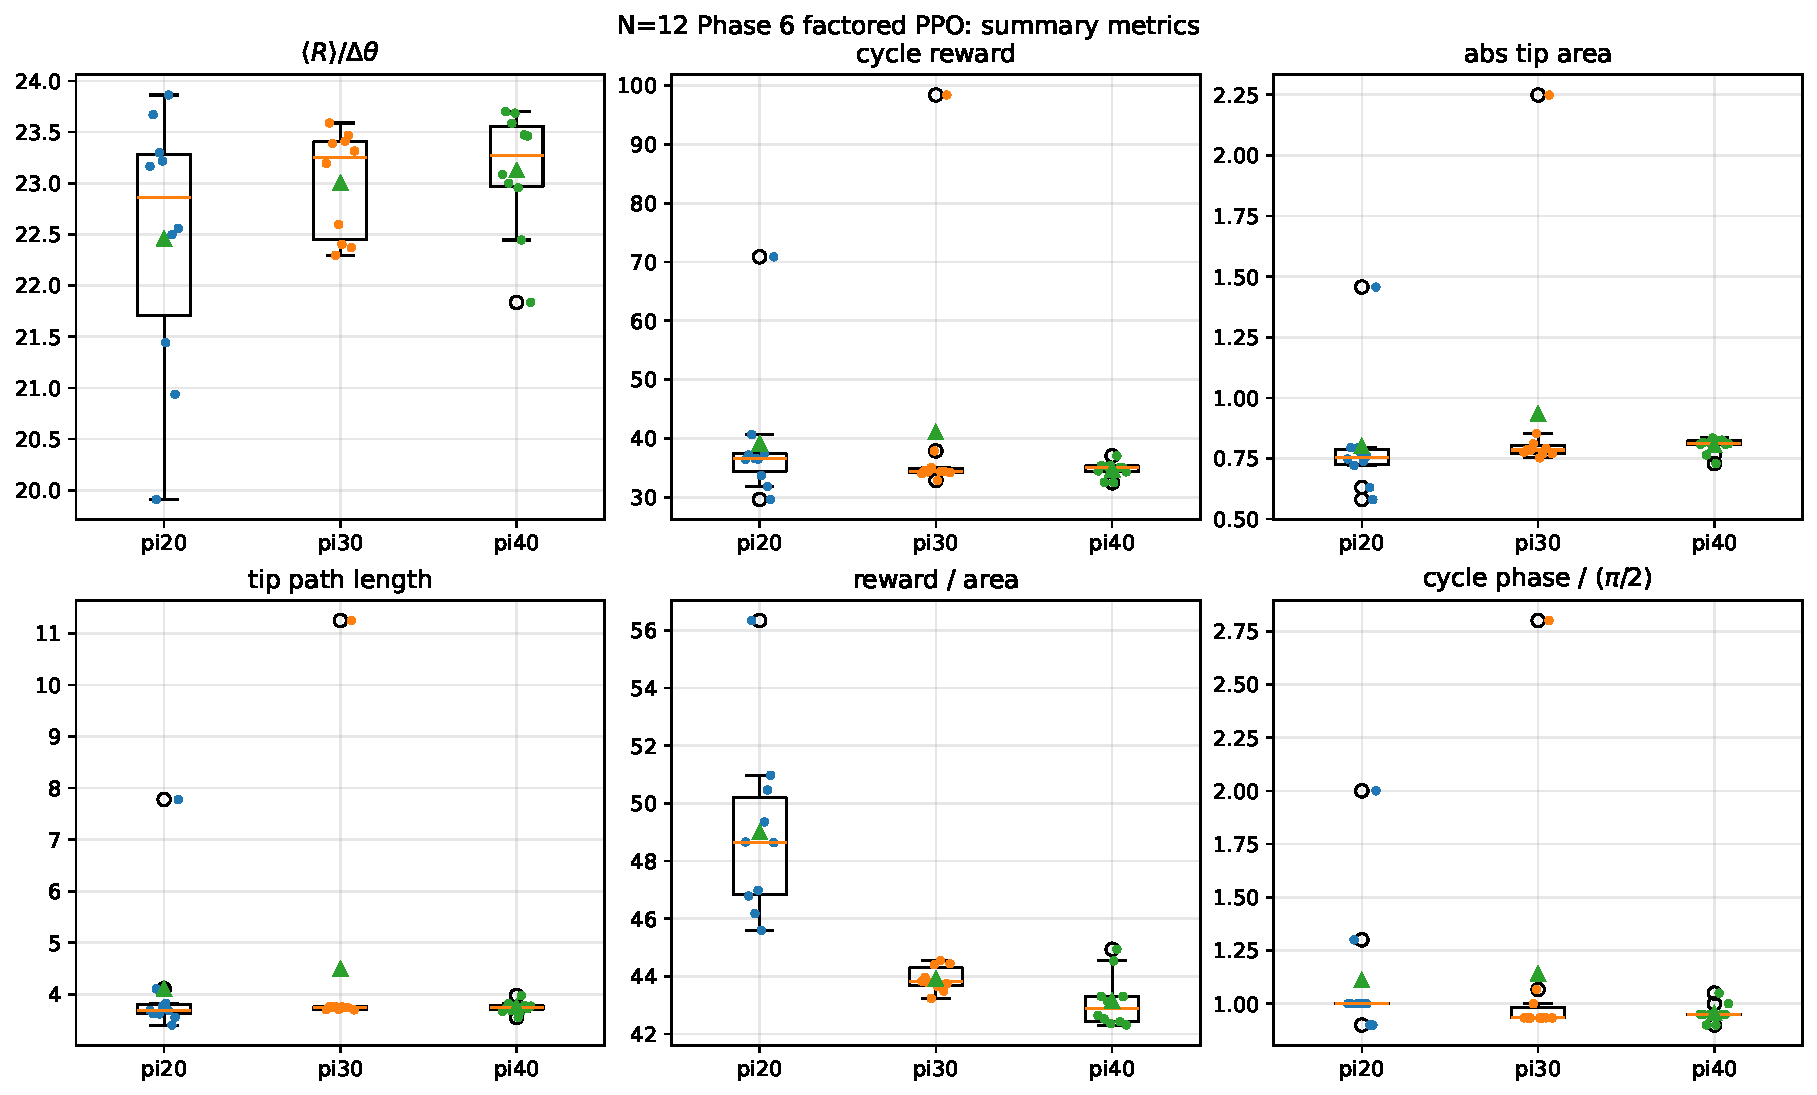
\includegraphics[width=\textwidth]{figs/phase6/fig01_summary_metrics.pdf}
    \caption{
    Summary metrics for the $N=12$ Phase 6 factored PPO sweep at
    $\Delta\theta=\pi/20$, $\pi/30$, and $\pi/40$.  Each case includes ten
    seeds.  The rescaled mean reward $\langle R\rangle/\Delta\theta$ is nearly
    constant under refinement, while the cycle reward, tip area, and tip path
    length remain clustered around comparable values.  The large outliers in
    cycle reward, area, path length, and cycle phase correspond to
    commensurate repeated-cycle solutions rather than wrong-orientation
    failures.
    }
    \label{fig:phase6-n12-summary}
\end{figure}

Table~\ref{tab:phase6-n12-aggregate} gives the corresponding aggregate
statistics.  The modal cycle lengths shift from about $L=10$ at $\pi/20$ to
$L=14$--$15$ at $\pi/30$ and $L=19$--$20$ at $\pi/40$, consistent with a
physical stroke duration close to $\pi/2$ in angular phase.

\begin{table}[htbp]
    \centering
    \small
    \caption{
    Aggregate statistics for the $N=12$ Phase 6 factored PPO sweep.  Entries
    are reported as median [min, max] over ten seeds, except for cycle lengths,
    which list the observed values.
    }
    \label{tab:phase6-n12-aggregate}
    \begin{adjustbox}{width=\textwidth}
    \begin{tabular}{llllllllll}
\toprule
case & runs & cycle lengths & mean reward / dtheta & cycle reward & tip area & tip path length & reward / area & cycle phase/(pi/2) & wrong orientation \\
\midrule
pi20 & 10 & 9, 10, 13, 20 & 22.86 [19.91, 23.86] & 36.53 [29.60, 70.87] & 0.754 [0.581, 1.457] & 3.687 [3.405, 7.778] & 48.65 [45.60, 56.34] & 1.00 [0.90, 2.00] & 0 \\
pi30 & 10 & 14, 15, 16, 42 & 23.25 [22.30, 23.59] & 34.36 [32.84, 98.39] & 0.785 [0.753, 2.249] & 3.754 [3.699, 11.249] & 43.81 [43.23, 44.55] & 0.93 [0.93, 2.80] & 0 \\
pi40 & 10 & 18, 19, 20, 21 & 23.27 [21.84, 23.70] & 35.02 [32.45, 37.02] & 0.813 [0.729, 0.834] & 3.750 [3.553, 3.976] & 42.89 [42.31, 44.94] & 0.95 [0.90, 1.05] & 0 \\
\bottomrule
\end{tabular}

    \end{adjustbox}
\end{table}

Figure~\ref{fig:phase6-n12-modal-strokes} shows representative modal strokes
for the three angular resolutions.  For each case, the plotted seed is the
median seed among the modal cycle-length class.  The cumulative spatial angle
diagnostic,
\[
    \Theta_j(t)=\sum_{m\leq j}\phi_m(t),
\]
provides a compact view of the evolving chain shape.  Across angular
refinements, the modal strokes show a similar repeating pattern in
$\Theta_j(t)$ and a similar reward rhythm over four cycles.

\begin{figure}[htbp]
    \centering
    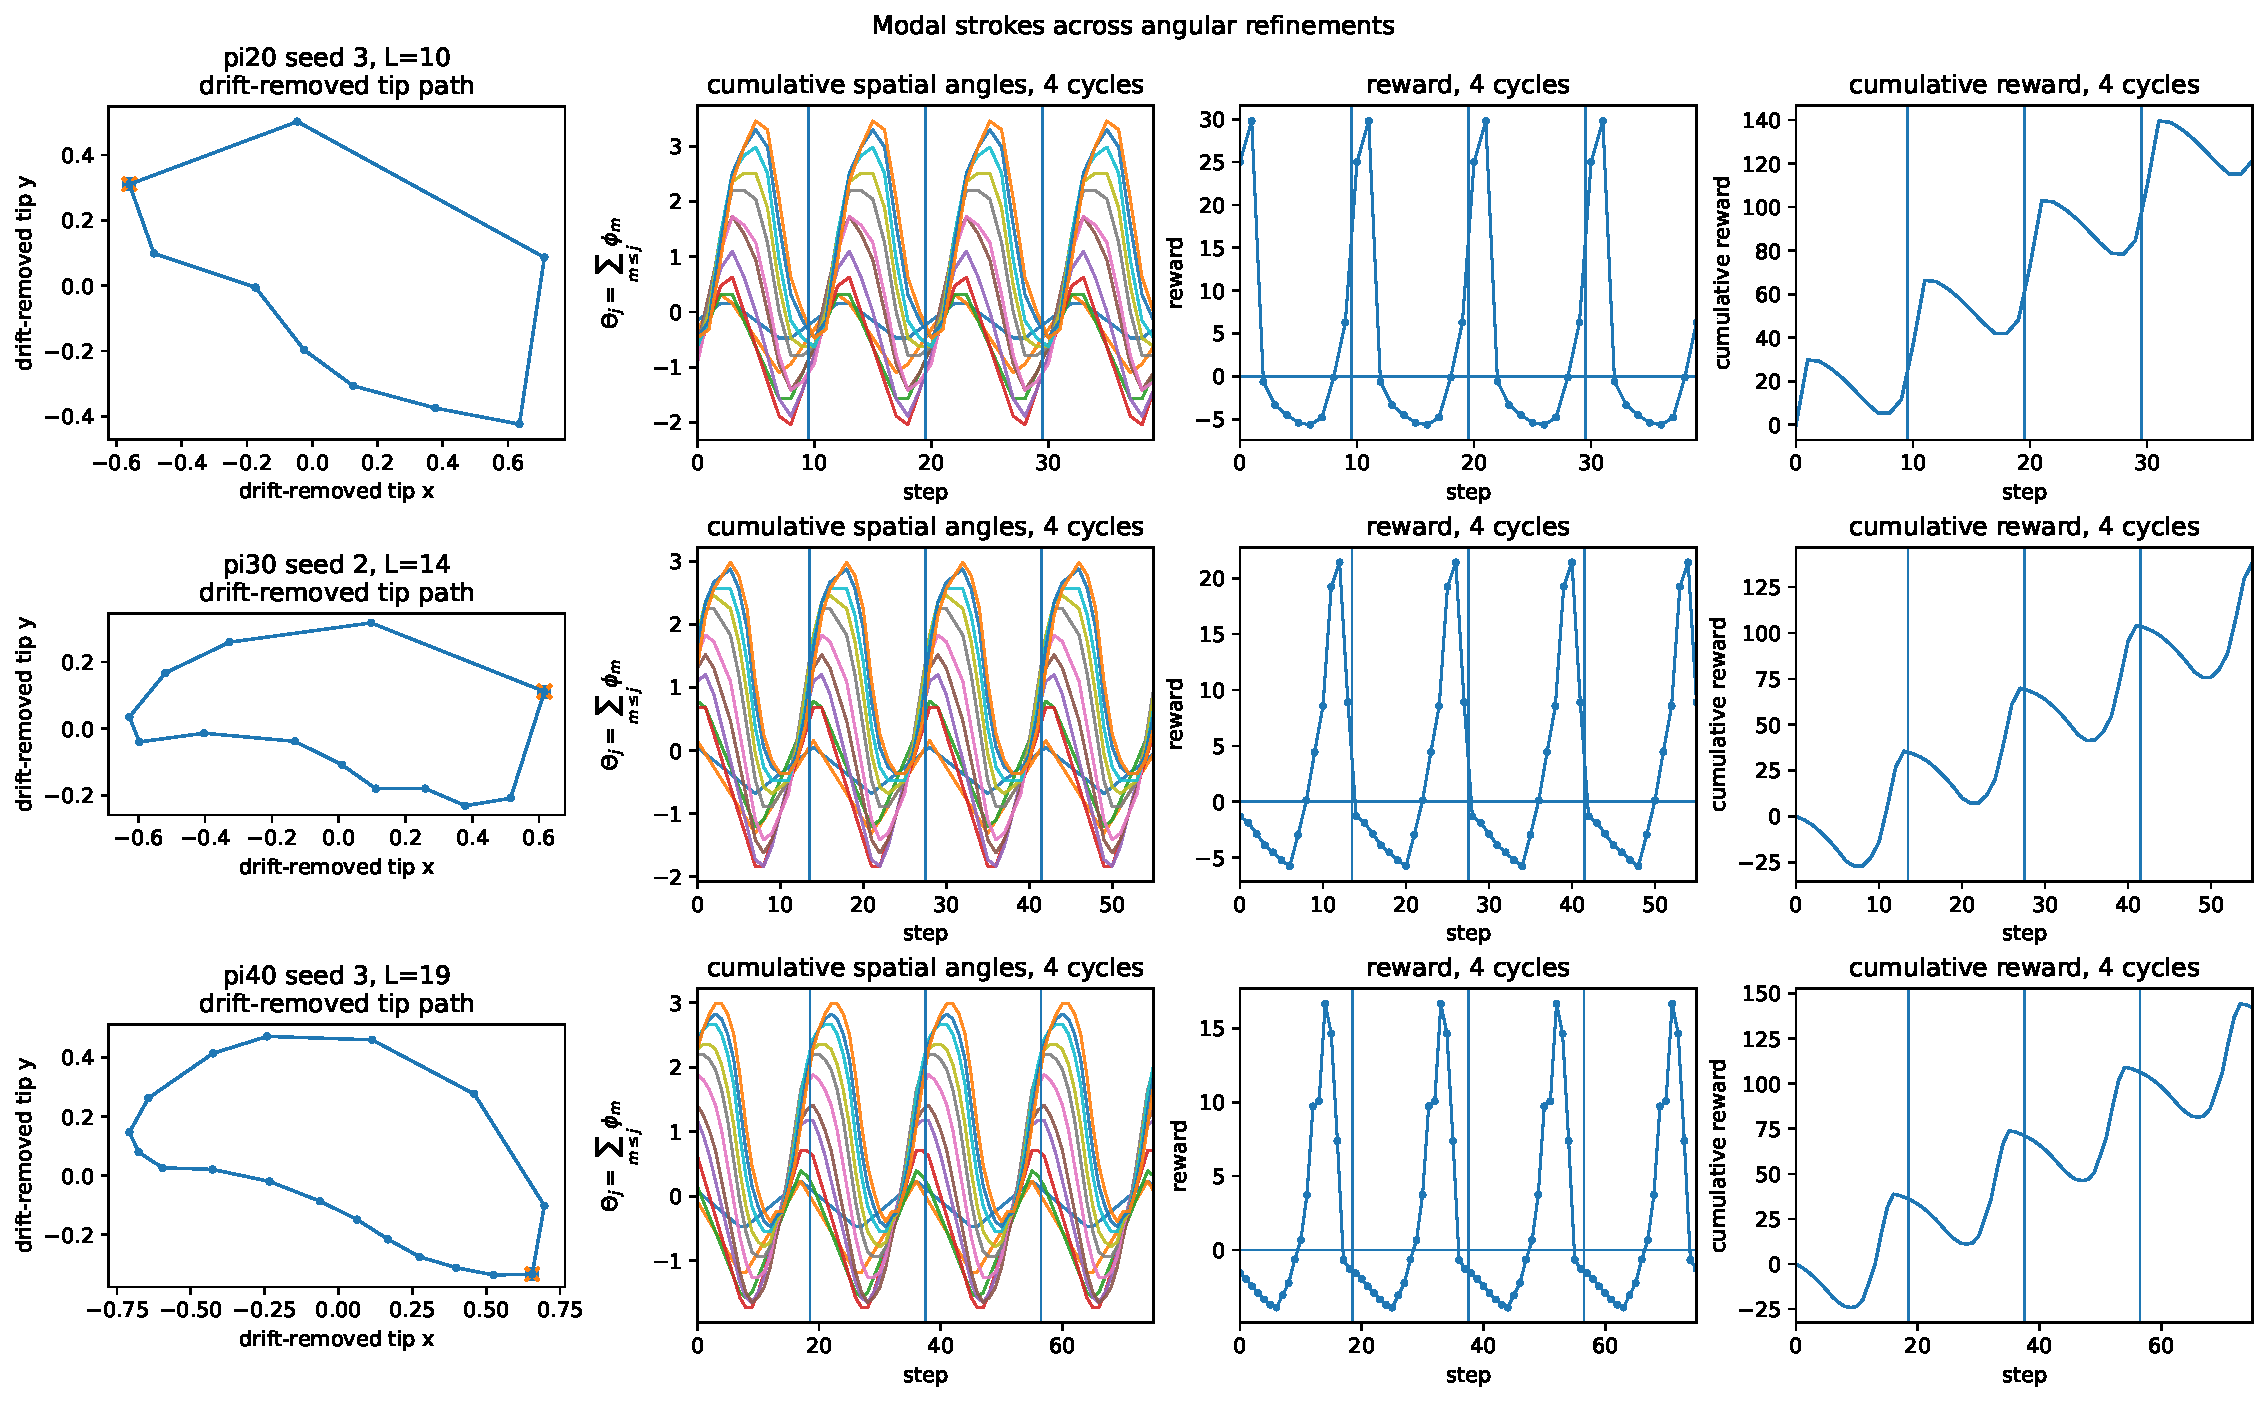
\includegraphics[width=\textwidth]{figs/phase6/fig02_modal_strokes_summary.pdf}
    \caption{
    Representative modal strokes for the $N=12$ Phase 6 factored PPO sweep.
    Rows correspond to $\Delta\theta=\pi/20$, $\pi/30$, and $\pi/40$.
    Columns show the drift-removed tip path, cumulative spatial angles
    $\Theta_j(t)=\sum_{m\leq j}\phi_m(t)$ over four cycles, reward over four
    cycles, and cumulative reward over four cycles.  The modal strokes exhibit
    a consistent body-shape rhythm and reward timing across angular
    refinements.
    }
    \label{fig:phase6-n12-modal-strokes}
\end{figure}

Table~\ref{tab:phase6-n12-modal} records the modal seeds used in
Figure~\ref{fig:phase6-n12-modal-strokes}.  The cycle rewards and geometric
metrics are similar across refinements, while the mean reward scales with the
angular step size.

\begin{table}[htbp]
    \centering
    \small
    \caption{
    Metrics for the representative modal seeds used in
    Figure~\ref{fig:phase6-n12-modal-strokes}.
    }
    \label{tab:phase6-n12-modal}
    \begin{adjustbox}{width=\textwidth}
    \begin{tabular}{lllllllll}
\toprule
case & seed & L & phase length & mean reward & cycle reward & tip area & tip path & reward/area \\
\midrule
pi20 & 3 & 10 & 1.57 & 3.66 & 36.6 & 0.793 & 3.62 & 46.2 \\
pi30 & 2 & 14 & 1.47 & 2.45 & 34.3 & 0.783 & 3.76 & 43.8 \\
pi40 & 3 & 19 & 1.49 & 1.85 & 35.2 & 0.816 & 3.71 & 43.1 \\
\bottomrule
\end{tabular}

    \end{adjustbox}
\end{table}

Some seeds converged to longer detected cycles.  These appear to be
commensurate repeated versions of the same underlying gait rather than distinct
failure modes.  In particular, the $\pi/20$ seed with $L=20$ is approximately
a two-cycle repeat of the modal $L=10$ branch, while the $\pi/30$ seed with
$L=42$ is approximately a three-cycle repeat of the modal $L=14$ branch.
Table~\ref{tab:phase6-n12-commensurate} summarizes these cases.

\begin{table}[htbp]
    \centering
    \small
    \caption{
    Commensurate-cycle interpretation of the long-cycle seeds.  The long
    cycles have cycle reward, tip area, and path length approximately
    proportional to the number of repeated modal strokes, while reward per area
    remains comparable.
    }
    \label{tab:phase6-n12-commensurate}
    \begin{adjustbox}{width=\textwidth}
    \begin{tabular}{llllllllllllll}
\toprule
case & seed & pick & L & phase length & cycle reward & tip area & tip path & reward/area & interpretation & L / modal & cycle reward / modal & tip area / modal & tip path / modal \\
\midrule
pi20 & 3 & modal\_L\_median & 10 & 1.57 & 36.6 & 0.793 & 3.62 & 46.2 & modal branch & 1 & 1 & 1 & 1 \\
pi20 & 9 & longest\_cycle & 20 & 3.14 & 70.9 & 1.46 & 7.78 & 48.6 & 2x repeat of L=10 branch & 2 & 1.94 & 1.84 & 2.15 \\
pi30 & 2 & modal\_L\_median & 14 & 1.47 & 34.3 & 0.783 & 3.76 & 43.8 & modal branch & 1 & 1 & 1 & 1 \\
pi30 & 8 & longest\_cycle & 42 & 4.4 & 98.4 & 2.25 & 11.2 & 43.7 & 3x repeat of L=14 branch & 3 & 2.87 & 2.87 & 2.99 \\
\bottomrule
\end{tabular}

    \end{adjustbox}
\end{table}

Finally, the finest angular resolution, $\Delta\theta=\pi/40$, gave the
cleanest cluster of results.  The selected $\pi/40$ seeds in
Table~\ref{tab:phase6-n12-pi40} span the worst, median, best, and longest-cycle
examples, yet all have similar cycle rewards, tip areas, path lengths, and
reward-per-area values.  This supports the interpretation that the learned
$N=12$ factored-policy stroke is robust at the finest tested resolution.

\begin{table}[htbp]
    \centering
    \small
    \caption{
    Selected $\Delta\theta=\pi/40$ seeds illustrating robustness of the
    learned $N=12$ factored-policy stroke.
    }
    \label{tab:phase6-n12-pi40}
    \begin{adjustbox}{width=\textwidth}
    \begin{tabular}{lllllllll}
\toprule
pick & seed & L & phase length & mean reward & cycle reward & tip area & tip path & reward/area \\
\midrule
worst\_mean & 9 & 20 & 1.57 & 1.71 & 34.3 & 0.811 & 3.77 & 42.3 \\
median\_mean & 8 & 19 & 1.49 & 1.84 & 35 & 0.809 & 3.72 & 43.3 \\
best\_mean & 1 & 19 & 1.49 & 1.86 & 35.4 & 0.817 & 3.73 & 43.3 \\
longest\_cycle & 6 & 21 & 1.65 & 1.76 & 37 & 0.824 & 3.98 & 44.9 \\
\bottomrule
\end{tabular}

    \end{adjustbox}
\end{table}

Overall, the $N=12$ Phase 6 results provide strong evidence that the
factored-action PPO formulation learns a coherent, resolution-consistent
stroke.  The main remaining ambiguity is not wrong orientation or policy
failure, but the appearance of commensurate repeated cycles in some seeds.

\section{Model summary and current stopping point}

The Phase 6 results provide a useful stopping point because they identify a specific model and parameter regime that succeeds robustly at $N=12$.  The successful setup is not a substantially new physical model relative to the earlier PPO scale-up.  The environment still uses the same relative-angle state variables, the same reward convention based on forward displacement, the same wall/contact safeguards, and the same post-hoc cycle diagnostics based on reward, tip area, tip path length, and reward per area.  The PPO policy is still the standard \texttt{MlpPolicy} with the same basic training configuration used throughout the validation and scale-up runs.

The main methodological change from Phase 5 is the action representation.  In Phase 5, the policy used a monolithic categorical action space consisting of all nonzero vectors in
\[
{-1,0,1}^N,
\]
so the number of actions was $3^N-1$.  In Phase 6, this is replaced by a factored action space,
\[
a_j \in {-1,0,1}, \qquad j=1,\ldots,N,
\]
implemented as one ternary decision per joint.  This changes the policy output structure from one large categorical choice to $N$ coupled ternary choices.  The global no-op action is technically available in the factored representation, but in the successful large-$N$ runs considered here the measured no-op fraction is zero.  Thus the learned policies are not exploiting the no-op option.

The second change is geometric rather than algorithmic.  The fixed-radius model with $r=0.05$ becomes invalid as $N$ increases because adjacent bead spacing scales like $1/N$.  Phase 6 therefore uses the scaled-radius branch
\[
r=\frac{0.4}{N},
\]
which agrees with the fixed-radius value at $N=8$ and preserves a constant relative thickness as the chain is refined.  This scaling makes the $N=10$ and $N=12$ experiments geometrically valid while leaving the rest of the reward and learning setup unchanged.

For the final $N=12$ comparison, we used factored-action PPO with
\[
r=\frac{0.4}{N}, \qquad
\Delta\theta \in {\pi/20,\pi/30,\pi/40},
\]
and $6\times 10^6$ training steps per seed.  The PPO hyperparameters were held fixed:
\[
\gamma=0.99,\qquad
n_{\rm steps}=2048,\qquad
{\rm batch\ size}=256,\qquad
n_{\rm epochs}=10,
\]
\[
{\rm learning\ rate}=3\times 10^{-4},\qquad
{\rm clip\ range}=0.2,\qquad
{\rm ent_coef}=0.
\]
Thus the $\pi/40$ result should be read as a success of this specific factored-action, scaled-radius PPO model, rather than as the result of additional reward shaping or exploration bonuses.

The strongest final result is the $N=12$, $\Delta\theta=\pi/40$ sweep.  All ten seeds produced positive coherent strokes, with no wrong-orientation failures and no no-op use.  The cycle lengths were tightly clustered, $L=18,19,20,21$, and the median diagnostics were
\[
\langle R\rangle \approx 1.83,\qquad
\frac{\langle R\rangle}{\Delta\theta} \approx 23.27,\qquad
R_{\rm cyc} \approx 35.02,
\]
\[
A_{\rm tip} \approx 0.81,\qquad
P_{\rm tip} \approx 3.75,\qquad
\rho=\frac{R_{\rm cyc}}{A_{\rm tip}} \approx 42.89.
\]
The rescaled mean reward $\langle R\rangle/\Delta\theta$, cycle reward, tip area, and tip path length are all consistent with the coarser $\pi/20$ and $\pi/30$ sweeps after accounting for commensurate repeated-cycle closures.  The representative modal strokes also show the same qualitative cumulative-angle rhythm and reward timing across angular refinements.

This gives a clean current conclusion: with factored actions, scaled radius $r=0.4/N$, the original displacement-based reward, and otherwise standard PPO hyperparameters, the model can learn robust positive-pumping strokes at $N=12$ and $\Delta\theta=\pi/40$.  At this point the main action-space and geometric bottlenecks have been controlled well enough to obtain coherent large-$N$ strokes.  The remaining long-cycle cases are best interpreted as commensurate closures of the same underlying stroke family, not as failures.  Thus the $N=12$, $\pi/40$ sweep is a successful stopping point for the present model specification.

\paragraph{Discussion point: scaled radius and regularization.}
One useful interpretation of the scaled-radius branch is that it is not a collision-softening device, but rather a self-similar geometric scaling.  In the environment, the same radius $r$ enters the wall/contact safeguards and, when $\epsilon$ is not explicitly specified, also sets the regularized-Stokeslet length scale through $\epsilon=1.5r$.  Thus for the scaled-radius choice
\[
r=\frac{0.4}{N},
\]
the segment length $\ell=1/N$, bead radius, contact threshold, and regularization length satisfy
\[
\frac{r}{\ell}=0.4,\qquad
\frac{2.2r}{\ell}=0.88,\qquad
\frac{\epsilon}{\ell}=0.6.
\]
These dimensionless ratios are fixed as $N$ changes.  In this sense, the scaled-radius branch prevents the artificial relative thickening that occurs under fixed $r=0.05$, where $r/\ell=rN$ increases with $N$ until the reset geometry becomes invalid.  The $N=12$, $\Delta\theta=\pi/40$ results should therefore be read as a success of a self-similar factored-action, scaled-radius model, not as a softened-collision artifact.  A caveat for future cross-$N$ comparisons is that holding $r/\ell$ and $\epsilon/\ell$ fixed does not imply exact hydrodynamic invariance with $N$: the absolute regularization length still decreases relative to the total swimmer length, so slow residual trends in quantities such as displacement, reward-per-area, or efficiency may reflect regularized-Stokeslet/slender-body effects rather than learning failure.



\end{document}
